\documentclass{../guide}

\usepackage{url}

\newcounter{stepcounter}

\newcommand{\newstep}[1]{\stepcounter{stepcounter}\section{Step \thestepcounter : #1}}

\title{Le guide de l'installeur galactique}
\author{Benoît Legat}

\begin{document}

\maketitle

\section{Prise d'informations}
\subsection{L'architecture}
\begin{itemize}
  \item ARM ou x86 ? Sûrement x86.
  \item 64-bits ou 32-bit ? 64-bit s'il est récent mais autant s'en assurer.
\end{itemize}

Comment savoir ?
\subsubsection{Sur Windows}
\paragraph{Windows XP}
Clique-droit sur ``My computer'' -> ``Properties''. Dans la catégorie ``System'', si il est écrit ``x64 edition'', c'est la version 64 bit, si vous ne voyez pas ``64'' quelque part, ça veut dire que c'est du 32bits.
\paragraph{Windows Vista/7}
Même chose que Windows XP, mais il sera explicitement écrit ``32-bit operating system'' ou ``64-bit operating system''.
\paragraph{Windows 8.1}
\todo[inline]{TODO}
\paragraph{Windows 10}
\todo[inline]{TODO}
\subsubsection{Sous MAC}
Ils sont tous 64 bits depuis 2008… Si vous voyez un tout veil ordi, regardez le type de processeur: Cliquez sur la pomme en haut à gauche $\to$ ``About this mac'', si le processeur est un ``Intel Core Solo'' ou ``Intel Core Duo'', c'est du 32-bit.
\subsubsection{Sur Linux}
\verb|i386| veut dire 32-bit et \verb|x86_64| veut dire 64-bit.
\begin{minted}{bash}
$ uname -a
\end{minted}

\subsection{SecureBoot}
Aller dans le start menu et lancer powershell en Administrator (clique droit sur l'app et sélectionner ``Run as Administrator'').
\begin{minted}{bash}
ms$ Confirm-SecureBootUEFI
\end{minted}
3 réponses possibles:
\begin{description}
  \item[True] Il y a Secure boot et il est Activé Enabled
  \item[False] Il y a Secure boot et il est Désactivé
  \item[Cmdlet not supported on this platform] Le système ne supporte pas Secure boot certaines étapes de ce guide sont donc peut-être superflues.
\end{description}

\subsection{Méthode de partitionnement}
GPT ou MBR.

Comment savoir ? \todo{TODO}
As a rule of thumb, si c'est Windows 8 ou plus c'est GPT.

\subsection{Repartitionnement}
Quels est la taille de la partition et les partitions présentes ?
\subsubsection{Sous Windows}
Aller dans le ``Gestionnaire de Disques''.
\paragraph{Windows 7 ou moins}
Clique droit sur ``My computer'' -> ``Manage''.
\paragraph{Windows 8 ou plus}
Clique droit sur menu démarrer -> ``Gestionnaire de disque''.
\subsubsection{Sous MAC}
\todo[inline]Utiliser l'''Utilitaire de Disque''.
\subsubsection{Sous Linux}
GParted ou plus rapide:
\begin{minted}{bash}
$ lsblk
\end{minted}

\section{Choix à faire avec le client}

\subsection{Quelle distribution ?}
Si ils demandent, ce qu'ils veulent (tant qu'on a l'ISO…), mais par défaut, Ubuntu. Pas besoin de leur faire peur inutilement !
Eventuellement, juste dire : ``Je vais installer Ubuntu''. Si ils veulent autre chose, ils réagiront. :)
Si il y a SecureBoot, utilisez Ubuntu 15.04 pour avoir moins d'ennuis, sinon mettez Ubuntu 14.04.3 pour qu'ils aient l'LTS.

\subsection{Quel place est-ce que le client veut donner ?}
Pour Linux, la taille de \verb|/|: minimum \SI{20}{GB} mais c'est short, \SI{32}{GB} c'est mieux, \SI{42}{GB} pour être tranquille.

Faire une SWAP entre \SI{2}{GB} et \SI{4}{\giga B}.

\subsection{Faire une partition home séparée ou pas ?}
Il y a deux cas de figures possibles:
\begin{enumerate}
  \item SWAP et \verb|/|
  \item SWAP, \verb|/home| et \verb|/|
\end{enumerate}

L'avantage de la deuxième c'est que si l'OS crash ou si il le client veut installer une autre distro ou une fresh install au lieu d'une update, en faisant l'install en demandant de ne pas reformatter la partition \verb|/home|, il n'y a que l'OS et les applications qui sont overwritten et les données restes inchangées.

Le désavantage de la deuxième c'est qu'il faut choisir la taille du \verb|/home| et \verb|/| maintenant et s'y tenir.
Seulement, la taille de \verb|/| n'est pas vraiment variable, on met souvent \SI{42}{GB} à \verb|/| et le reste à \verb|/home|.

\newstep{Défragmenter}
Idéalement ça doit déjà avoir été fait normalement...
C'est optionnel mais ça permet de plus diminuer la taille de Windows en Step 3.

\newstep{Désactiver le Fast Boot}
Pour éviter d'avoir des ennuis avec Windows qui boot pas et surtout, si on veut avoir accès aux paritions de Windows depuis Ubuntu,
il faut désactiver le Fast Boot depuis Windows.
Ne pas confondre avec la désactivation du Fast Boot depuis le BIOS !

Il faut aller dans:
Control Panel $\to$ Power Options $\to$ Choose what the power button does
Panneau de configuration $\to$ Choisir les options d'alimentation $\to$ Choisir ce que le bouton fait
Puis cliquer sur ``Change settings that are currently unavailable''.
On devrait voir:
\begin{center}
  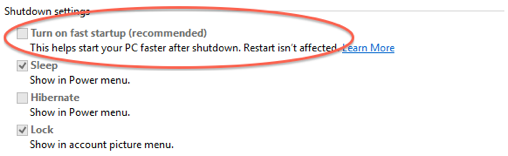
\includegraphics[scale=0.5]{fastboot.png}
\end{center}

Il faut aussi désactiver l'hibernation
\begin{minted}{bash}
  powercfg.exe -h off
\end{minted}

\newstep{Diminuer la taille de Windows}
Lancer l'application \verb|compmgmt.msc| sur Windows.

En MBR, s'il y a déjà 4 partitions il va falloir en supprimer une..
Il faut redimensionner Windows \emph{depuis Windows}.
C'est normal qu'il prenne du temps à calculer l'espace qu'il autorise à réduire et c'est normal que ce soit moins que l'espace libre.

Surtout ne pas virer la partition EFI (si on vire Windows, il faut la créer soit même \url{https://help.ubuntu.com/community/UEFI#Creating_an_EFI_partition}).

Créer un partition Ubuntu avec la taille choisie (la créer sur Windows évite certains problèmes).

\newstep{Rebooter dans l'UEFI}
Appuyer sur shift quand vous cliquez sur le bouton ``Redémarrer'' puis aller dans Troubleshoot puis UEFI Firmware Settings.

\newstep{Chipoter dans l'UEFI}
\begin{itemize}
  \item Laisser Secure Boot enabled (si ça marche pas, désactivez le et faite un launchpad bug pour le package ship).
  \item Disable Fast Boot.
  \item Le ``Boot Mode'' doit être en ``CSM (Compatibility Support Module) et pas ``UEFI Boot''. (C'est pour que l'UEFI apparaisse comme un BIOS)
  \item Enable ``UEFI Boot''. Il ne faut surtout pas booter en Legacy !
\end{itemize}
Mettre l'USB en priorité dans l'ordre de Boot.
Si l'USB n'est pas proposé, essayer de rebooter après avoir désactivé le Secure Boot.

Il se peut qu'il faille créer la Boot Entry soi-même (e.g. ASUS),
pour cela, il faut le faire pointer vers \verb|/boot/BOOTx86_64.efi|.

\subsection{Remarque sur le SecureBoot}
Ce n'est pas requis de désactiver SecureBoot dans le firmware pour Ubuntu 12.04.2 (64 bit versions) et plus récente
si l'ordi a la ``recommended Microsoft Third-Party Marketplace keys'' dans son firmware.
S'il y a un problème, il faut déclarer un launchpad bug dans le shim package.
Cependant, on doit dans tous les cas désactiver le SecureBoot après l'étape Boot Repair.

\newstep{Rebooter}
Maintenant, on reboot et ça devrait booter sur la clef (si ça ne marche pas, vous être autorisé à pleurer).

Choisir ``Try ...'' au lieu de ``Installer directemen't' pour avoir GParted.

\newstep{Créer les partitions}
Créer les partitions comme choisi au préalable avec le client.
Si c'est Windows 8 ou plus, faites aussi une Partition EFI de \si{250}{MB}, pour le format choisissez ``EFI boot partition''.
Si cette option ne s'affiche pas, vérifiez que vous avez booté votre clef USB avec le UEFI enabled et si ça marche toujours pas, vérifiez que votre clef USB a été faite avec \verb|dd| (voir \url{http://askubuntu.com/questions/562982/ubuntu-14-04-single-boot-with-uefi-mode-enabled/563004#563004}).
\todo[inline]{Boot partition?}

\newstep{Se connecter}
Wifi c'est bien, Ethernet, c'est mieux !
Brancher aussi le PC, si ce n'est pas encore fait.

\newstep{Lancer l'installation}
Double cliquer sur les partitions ext4 créées pour qu'elles soient utilisées.
Ne pas reformater la partition \verb|/home| s'il y a des données (e.g. reinstall).
Pour l'installation du Boot Loader, choisissez \verb|/dev/sda| pour Windows 7 ou moins (normalement choisi par défaut)
et la partition de type ``EFI'' sinon.

\newstep{Rebooter}
Checkez si Windows marche.
Checkez si Linux marche:
Checker qu'il est bien en EFI avec
\begin{minted}{bash}
$ [ -d /sys/firmware/efi ] && echo "Installed in EFI mode" || echo "Installed in Legacy mode"
\end{minted}
\begin{itemize}
  \item Wifi
  \item Son
  \item Luminosité
  \item ...
\end{itemize}
Démarrez ``Additionnal drivers'' pour installer des drivers supplémentaires (e.g. wifi, carte graphique).

\subsection{Drivers graphiques}
To know which are your graphics cards, do
\begin{minted}{bash}
$ lspci | grep -e "VGA\|3D\|Display"
\end{minted}
or
\begin{minted}{bash}
$ xrandr --listproviders # may not show cards that are off or for which the driver is not loaded
\end{minted}

\subsection{Codecs}
To be able to play most audio and video formats, install Ubuntu Restricted Extras
\begin{minted}{bash}
$ sudo apt-get install ubuntu-restricted-extras
\end{minted}

I suggest to also install the unrestricted versions of libavformat and libavcodec so you don't encounter issues with missing codecs when trying to use some video editors or transcoders
\begin{minted}{bash}
$ sudo apt-get install libavformat-extra-53 libavcodec-extra-53
\end{minted}

Encrypted DVD playback: the Medibuntu repository no longer exists and while most packages in the archive are obsolete or unnecessary because most are now in the official Ubuntu repository or have better equivalents, livdvdcss is still required for playing encrypted DVDs.

You can enable encrypted DVD playback in Ubuntu 13.10 by using the following commands:
\begin{minted}{bash}
$ sudo apt-get install libdvdread4
$ sudo /usr/share/doc/libdvdread4/install-css.sh
\end{minted}


\section*{Sources}
\begin{itemize}
  \item \url{http://askubuntu.com/questions/221835/installing-ubuntu-on-a-pre-installed-windows-with-uefi}
  \item \url{https://help.ubuntu.com/community/UEFI}
  \item \url{http://askubuntu.com/questions/562982/ubuntu-14-04-single-boot-with-uefi-mode-enabled/563004#563004}
\end{itemize}

\section{Troubleshooting}

\subsection{YOUR COMPUTER BOOTS DIRECTLY TO WINDOWS}

This is a common problem and if you do not get a GRUB menu , re-installing or repairing grub will NOT HELP

Notice the "UEFI Boot Option Priority" or "Boot Option Menu" . Usually Windows is the default and Ubuntu (or as in the second picture elementary OS) will be an option.

Once you select Ubuntu on the UEFI boot menu you will then get a grub menu. You should be able to boot either Ubuntu or Windows from the grub menu.

Another issue that could make the system boot directly to Windows (without even showing the GRUB menu) is if either Windows took hold of the boot manager or after installing Ubuntu, the EFI partition was not properly configured for Windows. To solve this, simply go to Windows and open a terminal, then type the following (Need Administrative Privileges):
\begin{minted}{bash}
bcdedit /set {bootmgr} path \EFI\ubuntu\grubx64.efi
\end{minted}
This will configure the Windows Boot Manager to take into consideration the GRUB Boot Manager. This could still happen even after running the Boot Repair from within Ubuntu. So making sure that Windows reads the Ubuntu EFI partition, in case you are using an EFI boot system instead of the old BIOS will solve it.

\subsection{REPAIRING THE BOOT}
After finishing the installation, if you happen to have Windows 8 disabled from booting and it only boots to Ubuntu, do not worry. In Ubuntu after it boots, install Boot-Repair in Ubuntu by opening a Terminal and typing the following:

\begin{minted}{bash}
sudo add-apt-repository ppa:yannubuntu/boot-repair
sudo apt-get update
sudo apt-get install boot-repair
boot-repair
\end{minted}
Boot Repair will mention that we have some GRUB error, that we have an EFI system and that Ubuntu rocks. Since Ubuntu rocks (It does not work if Ubuntu does not rock!), just click on Apply so boot repair fixes everything. Now reboot and you should see Windows 8 and Ubuntu side by side.

For cases with rare booting problems, partitioning or using old hard drives on newer motherboard, your solution might be checking out FixParts (\url{http://www.rodsbooks.com/fixparts/}) which solves misaligned partitions and other partitioned type problems.

\end{document}
